
\begin{figure}
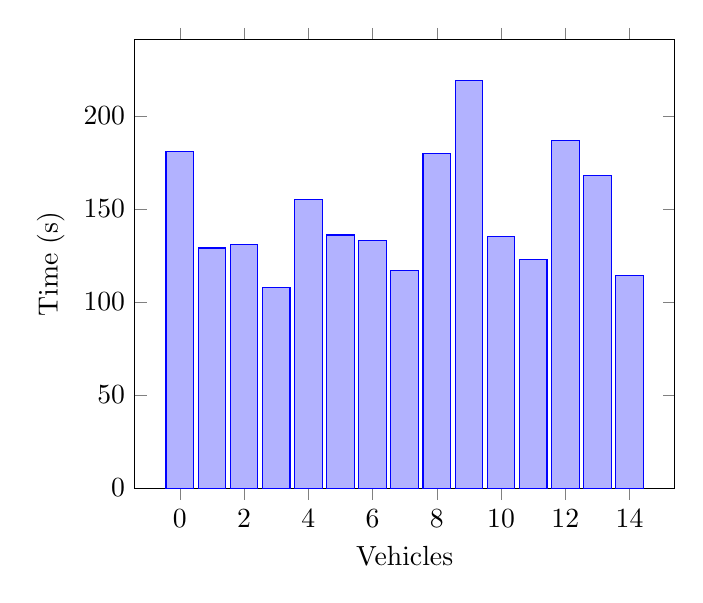
\begin{tikzpicture}
\begin{axis}[
legend style={anchor=west},
xlabel=Vehicles,
ylabel=Time (s),
ymin=0,
ybar,
]
\addplot coordinates {
(0, 181)
(1, 129)
(2, 131)
(3, 108)
(4, 155)
(5, 136)
(6, 133)
(7, 117)
(8, 180)
(9, 219)
(10, 135)
(11, 123)
(12, 187)
(13, 168)
(14, 114)
};

\end{axis}
\end{tikzpicture}
\label{tik:0:21_V, 20_V, 17_N, 15_S, 15_S.-30, 13_N, 13_N.-40, 11_N, 8_N, 7_N, 7_N.-60, 5_N, 4_N, 4_N.-60, 3_O}
\caption{0 percent diving with GSC on route $21_V, 20_V, 17_N, 15_S, 15_S.-30, 13_N, 13_N.-40, 11_N, 8_N, 7_N, 7_N.-60, 5_N, 4_N, 4_N.-60, 3_O$}
\end{figure}
